\documentclass[journal,12pt,twocolumn]{IEEEtran}

\usepackage{setspace}
\usepackage{gensymb}
\singlespacing
\usepackage[cmex10]{amsmath}

\usepackage{amsthm}

\usepackage{mathrsfs}
\usepackage{txfonts}
\usepackage{stfloats}
\usepackage{bm}
\usepackage{cite}
\usepackage{cases}
\usepackage{subfig}

\usepackage{longtable}
\usepackage{multirow}

\usepackage{enumitem}
\usepackage{mathtools}
\usepackage{steinmetz}
\usepackage{tikz}
\usepackage{circuitikz}
\usepackage{verbatim}
\usepackage{tfrupee}
\usepackage[breaklinks=true]{hyperref}
\usepackage{graphicx}
\usepackage{tkz-euclide}

\usetikzlibrary{calc,math}
\usepackage{listings}
    \usepackage{color}                                            %%
    \usepackage{array}                                            %%
    \usepackage{longtable}                                        %%
    \usepackage{calc}                                             %%
    \usepackage{multirow}                                         %%
    \usepackage{hhline}                                           %%
    \usepackage{ifthen}                                           %%
    \usepackage{lscape}     
\usepackage{multicol}
\usepackage{chngcntr}

\DeclareMathOperator*{\Res}{Res}

\renewcommand\thesection{\arabic{section}}
\renewcommand\thesubsection{\thesection.\arabic{subsection}}
\renewcommand\thesubsubsection{\thesubsection.\arabic{subsubsection}}

\renewcommand\thesectiondis{\arabic{section}}
\renewcommand\thesubsectiondis{\thesectiondis.\arabic{subsection}}
\renewcommand\thesubsubsectiondis{\thesubsectiondis.\arabic{subsubsection}}


\hyphenation{op-tical net-works semi-conduc-tor}
\def\inputGnumericTable{}                                 %%

\lstset{
%language=C,
frame=single, 
breaklines=true,
columns=fullflexible
}
\begin{document}


\newtheorem{theorem}{Theorem}[section]
\newtheorem{problem}{Problem}
\newtheorem{proposition}{Proposition}[section]
\newtheorem{lemma}{Lemma}[section]
\newtheorem{corollary}[theorem]{Corollary}
\newtheorem{example}{Example}[section]
\newtheorem{definition}[problem]{Definition}

\newcommand{\BEQA}{\begin{eqnarray}}
\newcommand{\EEQA}{\end{eqnarray}}
\newcommand{\define}{\stackrel{\triangle}{=}}
\bibliographystyle{IEEEtran}
\raggedbottom
\setlength{\parindent}{0pt}
\providecommand{\mbf}{\mathbf}
\providecommand{\pr}[1]{\ensuremath{\Pr\left(#1\right)}}
\providecommand{\qfunc}[1]{\ensuremath{Q\left(#1\right)}}
\providecommand{\sbrak}[1]{\ensuremath{{}\left[#1\right]}}
\providecommand{\lsbrak}[1]{\ensuremath{{}\left[#1\right.}}
\providecommand{\rsbrak}[1]{\ensuremath{{}\left.#1\right]}}
\providecommand{\brak}[1]{\ensuremath{\left(#1\right)}}
\providecommand{\lbrak}[1]{\ensuremath{\left(#1\right.}}
\providecommand{\rbrak}[1]{\ensuremath{\left.#1\right)}}
\providecommand{\cbrak}[1]{\ensuremath{\left\{#1\right\}}}
\providecommand{\lcbrak}[1]{\ensuremath{\left\{#1\right.}}
\providecommand{\rcbrak}[1]{\ensuremath{\left.#1\right\}}}
\theoremstyle{remark}
\newtheorem{rem}{Remark}
\newcommand{\sgn}{\mathop{\mathrm{sgn}}}
% \providecommand{\abs}[1]{\left\vert#1\right\vert}
% \providecommand{\res}[1]{\Res\displaylimits_{#1}} 
% \providecommand{\norm}[1]{\left\lVert#1\right\rVert}
% %\providecommand{\norm}[1]{\lVert#1\rVert}
% \providecommand{\mtx}[1]{\mathbf{#1}}
% \providecommand{\mean}[1]{E\left[ #1 \right]}
\providecommand{\fourier}{\overset{\mathcal{F}}{ \rightleftharpoons}}
%\providecommand{\hilbert}{\overset{\mathcal{H}}{ \rightleftharpoons}}
\providecommand{\system}{\overset{\mathcal{H}}{ \longleftrightarrow}}
	%\newcommand{\solution}[2]{\textbf{Solution:}{#1}}
\newcommand{\solution}{\noindent \textbf{Solution: }}
\newcommand{\cosec}{\,\text{cosec}\,}
\providecommand{\dec}[2]{\ensuremath{\overset{#1}{\underset{#2}{\gtrless}}}}
\newcommand{\myvec}[1]{\ensuremath{\begin{pmatrix}#1\end{pmatrix}}}
\newcommand{\mydet}[1]{\ensuremath{\begin{vmatrix}#1\end{vmatrix}}}
\numberwithin{equation}{subsection}
\makeatletter
\@addtoreset{figure}{problem}
\makeatother
\let\StandardTheFigure\thefigure
\let\vec\mathbf
\renewcommand{\thefigure}{\theproblem}
\def\putbox#1#2#3{\makebox[0in][l]{\makebox[#1][l]{}\raisebox{\baselineskip}[0in][0in]{\raisebox{#2}[0in][0in]{#3}}}}
     \def\rightbox#1{\makebox[0in][r]{#1}}
     \def\centbox#1{\makebox[0in]{#1}}
     \def\topbox#1{\raisebox{-\baselineskip}[0in][0in]{#1}}
     \def\midbox#1{\raisebox{-0.5\baselineskip}[0in][0in]{#1}}
\vspace{3cm}
\title{Assignment 1}
\author{Buereddy Varuni - EE18BTECH11005}
\maketitle
\newpage
\bigskip
\renewcommand{\thefigure}{\theenumi}
\renewcommand{\thetable}{\theenumi}
Download all latex-tikz codes from 
%
\begin{lstlisting}
https://github.com/varunireddy/-C-DS/blob/main/assignment1/assignment1.tex
\end{lstlisting}
\section{Problem}
Q41. An articulation point in a connected graph is a vertex such that removing the vertex and its incident edges disconnects the graph into two or more connected components.
Let T be a DFS tree obtained by doing DFS in a connected undirected graph G.
Which of the following options is/are correct?
\begin{enumerate}
    \item Root of T can never be an articulation point in G.
    \item Root of T is an articulation point in G if and only if it has 2 or more children.
    \item A leaf of T can be an articulation point in G
    \item If u is an articulation point in G such that x is an ancestor of u in T and y is a descendent of u in T, then all paths from x to y in G must pass through u.
\end{enumerate}
\section{Solution}
Answer : 2
\\
\textbf{Explanation}
\\
Option 2 - Root of T is an articulation point in G if and only if it has 2 or more children. Because, option 2 is an if and only if statement, we have to prove in both the ways. 
\\
\textbf{Case 1:- If root is articulation point then root will have 2 or more children}\\
A vertex is said to be an articulation point if its removal disconnects the graph into 2 or more components. If root is an articulation point. Removal of root node will disconnect the graph. And there is no path between the disconnected components. Therefore, while constructing the DFS tree for graph G, Root vertex is first visited and will have two or more children. 
\\  
\textbf{Case 2:- If root vertex has 2 or more children then it is articulation point}\\
Lets say in an undirected graph if root has 2 children then it is true that there is no path between the vertices in left sub-tree and right sub-tree of vertex V (w.r.t DFS traversal tree) because if there had been any path between the left and right sub-tree the in that case if we start with right child then before reaching to the root all the vertices in left sub-tree would have been visited and root had only single child but it is contradiction as root has 2 children and hence there can be no path between the left and right sub-tree of vertex V, thereby making it the ONLY vertex through which vertices in left and right sub-tree are connected.
\\ 
Therefore, Option 2 is correct which also implies Option 1 is wrong.\\
Option 3 - A leaf of T can be an articulation point in G
 This is FALSE because if some vertex is leaf of tree T then all the vertices to which it connects are already been visited which indicates that even without using this leaf vertex there exists path between all of its neighbors and hence it can not be an articulation point.
 \\
 Option 4 - In the figure 1 is the counter example, U is the articulation point in G. And also X is the ancestor of U and Y is the descendent of U. But all the paths from X and Y in G does not pass through U.
\\
Therefore, Option 2 is correct.\\

\begin{figure}
    \centering
    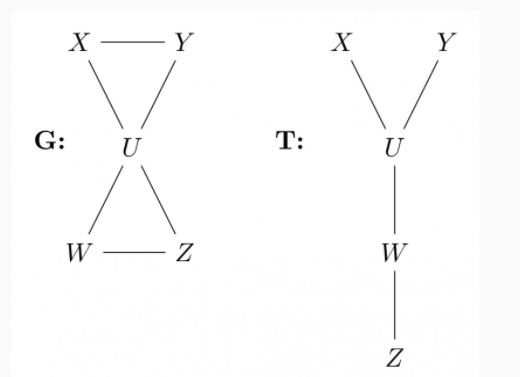
\includegraphics[scale=0.6]{assignment1.png}
    \caption{1}
    \label{fig: figure1}
\end{figure}
\textbf{Application in Electric circuits:-}\\
\textbf{KIRCHOFFS GRAPH:-}
An electrical circuit can be seen as a connected graph where the nodes of the
electrical circuit are the vertices of the graph and the wires of the electrical cricuit
are the edges of the graph. This will be named Kirchhoff or electrical graph. 
An articulation point in the electric circuit is the node when removed forms two or more different circuits. For example in the figure 2, the node A is the articulation point, which when removed disconnects the circuit.
\begin{figure}
    \centering
    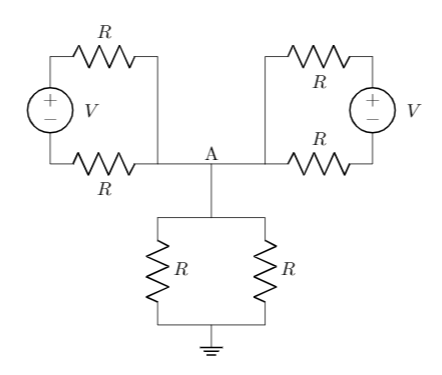
\includegraphics[scale=0.9]{circuit.PNG}
    \caption{2}
    \label{fig:figure2}
\end{figure}
\\
\section{Solving circuit equations using graphs}
\textbf{GRAPH:- } Graph is the set of ordered pair G=(V,E) of sets where  E=$\{\{x,y\}$ : x,y $\epsilon$ V$\}$
The elements of V are called vertices (or nodes) of the graph G and the elements of E are called edges. So in a graph a vertex set is a set of 
points $\{x_1,x_2,x_3,..,x_n\}$ and edge is a line which connects two points $x_i$ and $x_j$. Such graphs are called undirected graphs. A directed graph is similar to an undirected graph except the edge set E $\epsilon$ VxV.
\\
\textbf{ELECTRICAL CIRCUITS :-} An electrical circuit consists of internally connected elements viz resistors,capacitors,inductors,diodes, transistors etc.The behaviour of an electrical circuits generally depends upon two factors.
\begin{itemize}
    \item The characteristic of each of internally connected elements
    \item The rule by which they are connected together.
\end{itemize}
The second factor gives a relation between electrical circuits with graph theory. A two terminal electrical element can be represented by an edge $e_k$. Associate with each edge there are two variables $V_k(t)$ and $i_k(t)$. The variable $V_k(t)$ is called the edge voltage. The variable $i_k(t)$ is called the edge current.
\\
\textbf{Kirchhoff’s Current Law (KCL):-} For any lumped electrical network, at any time the net sum (taking into account the orientations) of all the currents leaving any node or vertex is zero. That is at $r^{th}$ vertex of the corresponding digraph,we must have
\begin{align}
    [A][I] = 0\\
    \sum_{k=1}^{e} a_{rk}i_k(t) = 0
\end{align}
Where $a_{rk}$ is the $rk^{th}$ entry of the incidence matrix A of G and 
$i_k(t)$ is the amount of current flowing through the $k^{th}$
edge of G.
\\
\textbf{Kirchhoff’s Voltage Law (KVL):-} For any lumped electrical network, at any time the net sum (taking into account the orientations) of the voltages around a loop (i.e. circuit) is zero. In terms of the corresponding digraph , for the $r^{th}$ circuit 
we must have
\begin{align}
    [B][V] = 0\\
    \sum_{k=1}^{e} b_{rk}v_k(t) = 0
\end{align}
Where $b_{rk}$ is the $rk^{th}$ entry of the circuit matrix B of G and 
$v_k(t)$ is the amount of voltage across the $k^{th}$
edge of G.
\\
\textbf{Application of graph theory in network equilibrium equations:}\\
Steps to be followed:-
\begin{enumerate}
    \item Find the equivalent graph of the circuit.
    \item Find the standard tree that passes through all the nodes and does not have any loops.
    \item Construct the tie-set matrix(B).
    \item Apply equivalent KCL for the graph. 
\end{enumerate}
Let a voltage $V_{sk}$ be in branch k having impedance $z_k$ and carrying current $i_k$, we can write $v_k$ = $z_ki_k$ + $V_{sk}$. In matrix form this can be written as [$V_b$] = [$Z_b$][$I_b$]+[$V_s$] where [$Z_b$] is the branch impedance matrix,[$I_b$] is the column vector of branch currents and [$V_s$] is the column vector of source voltage. Now Kirchhoff’s Voltage law in 
matrix form is given by
\begin{align}
    [B][V_b] = 0\\
    [B]\{[Z_b][I_b]+[V_s]\} = 0\\
    [B][Z_b][I_b] = -[B][V_s] \label{eq:equation1}
\end{align}
Consider the example circuit as shown in the figure.3. 
\begin{figure}
    \centering
    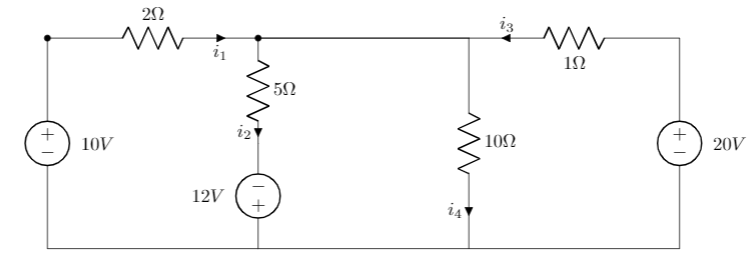
\includegraphics[scale=0.6]{example_circuit.PNG}
    \caption{3}
    \label{fig:example_circuit}
\end{figure}
The obtained equivalent graph is shown in the figure.4
\begin{figure}
    \centering
    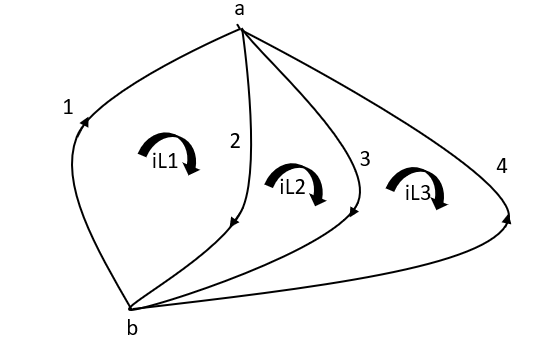
\includegraphics[scale=0.6]{example_graph.PNG}
    \caption{4}
    \label{fig:example_graph}
\end{figure}
\\
There are two vertices and four branches in the graph. We need to first find the B matrix(tie-set matrix). The size of matrix B is number of loops x number of branches(3x4).$B_{ij}$=1 if $j^{th}$ branch current is in the direction of $i^{th}$ loop current.\\
tie-set matrix = $B = \begin{bmatrix}
        1 & 1 & 0 & 0\\
        0 & -1 & 1 & 0\\
        0 & 0 & -1 & -1
        \end{bmatrix}
 $\\
 $B^T = \begin{bmatrix}
        1 & 0 & 0 \\
        1 & -1 & 0 \\
        0 & 1 & -1\\
        0 & 0 & -1
        \end{bmatrix}
 $\\
Now find the circuit impedance matrix [zb]. The size of [zb] is number of branches x number of branches(4x4),\\ $
zb = \begin{bmatrix}
    2 & 0 & 0 & 0\\
    0 & 5 & 0 & 0\\
    0 & 0 & 10 & 0\\
    0 & 0 & 0 & 1
 \end{bmatrix}
$\\
Vs is the external source matrix,
$Vs = \begin{bmatrix}
        -10 \\ -12 \\ 0 \\ -20 
 \end{bmatrix}
$\\
The loop currents $I_L$ has dimension (number of loops x 1) (3x1).\\
$I_L = \begin{bmatrix}
i_{L1} \\ i_{L2} \\ i_{L3}
\end{bmatrix}
$\\
From the equation.\ref{eq:equation1},

[B][$Z_b$][$B^T$][$I_L$] = -[B][$V_s$]\\
  $ \begin{bmatrix}
        2 & 5 & 0 & 0\\
        0 & -5 & 10 & 0\\
        0 & 0 & -10 & -1
    \end{bmatrix}
    \begin{bmatrix}
        1 & 0 & 0 \\
        1 & -1 & 0 \\
        0 & 1 & -1\\
        0 & 0 & -1
        \end{bmatrix}
 \begin{bmatrix}
i_{L1} \\ i_{L2} \\ i_{L3}
\end{bmatrix} = \begin{bmatrix}
22 \\ -12 \\ -20
\end{bmatrix}$\\
$\begin{bmatrix}
7 & -5 & 0\\
-5 & 15 & -10\\
0 & -10 & 11
\end{bmatrix}\begin{bmatrix}
i_{L1} \\ i_{L2} \\ i_{L3}
\end{bmatrix} = \begin{bmatrix}
22 \\ -12 \\ -20
\end{bmatrix}$

 Solving the above equation, we get
 \begin{align}
     i_{L1} = -1.2777 A\\
     i_{L2} = -6.188 A\\
     i_{L3} = -7.444 A
 \end{align}
\end{document}